\documentclass[11pt, oneside]{article}   	% use "amsart" instead of "article" for AMSLaTeX format
\usepackage{geometry}                		% See geometry.pdf to learn the layout options. There are lots.
\geometry{letterpaper}                   		% ... or a4paper or a5paper or ... 
%\geometry{landscape}                		% Activate for for rotated page geometry
%\usepackage[parfill]{parskip}    		% Activate to begin paragraphs with an empty line rather than an indent
\usepackage{graphicx}				% Use pdf, png, jpg, or eps§ with pdflatex; use eps in DVI mode
								% TeX will automatically convert eps --> pdf in pdflatex		
\usepackage{amssymb}
\usepackage{amsmath}
\usepackage{parskip}
\usepackage{color}
\usepackage{hyperref}

\title{Complex numbers:  inverse}
%\author{The Author}
%\section{}
%\subsection*{}
\date{}							% Activate to display a given date or no date

\graphicspath{{/Users/telliott_admin/Dropbox/Tex/png/}}
% \begin{center} 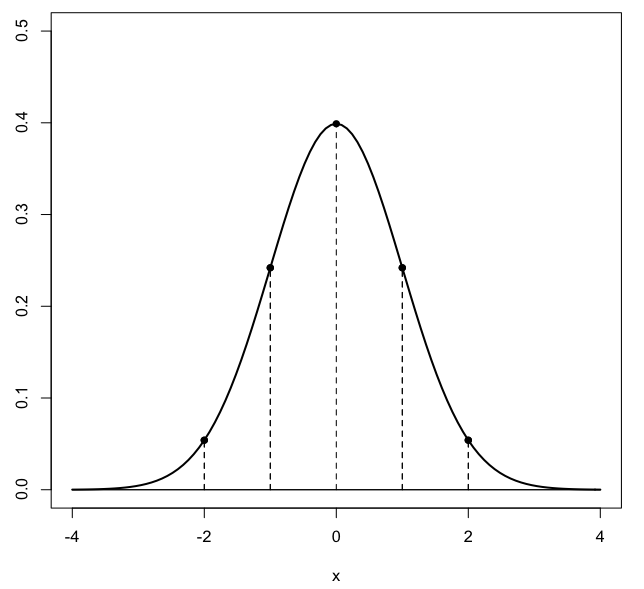
\includegraphics [scale=0.4] {gauss3.png} \end{center}
\begin{document}
\maketitle
\Large
Consider the complex number:
\[ z = x + iy \]
The complex conjugate of $z$ (called $z*$ or $\bar{z}$) is given by:
\[ z* = x - iy \]
The real part of $z*$ is the same as the real part of $z$, while the imaginary part has the signs switched.

The \emph{length} of $z$ squared is equal to $z$ multiplied by its complex conjugate
\[ zz* = (x + iy) (x - iy) \]
\[ =  x^2 - ixy + ixy -i^2y^2 \]
\[ = x^2 + y^2 \]
\[ = r^2 \cos^2 \theta + r^2 \sin^2 \theta \]
\[ = r^2   \]
Again, $r$ is the length of the ray from the origin to $z$ as plotted in the complex plane.
\[ r^2 = zz* \]
\[ r = \sqrt{zz*} \]
The point corresponding to $z*$ in the complex plane has the same overall distance from the origin and the same $x$-component as $z$, but the sign change on $y$ means that $z*$ is reflected across the $x$-axis from $z$.
\begin{center} 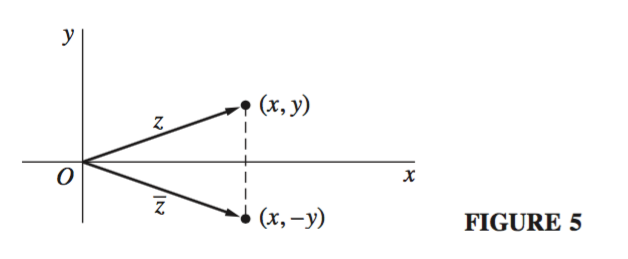
\includegraphics [scale=0.6] {Brown5.png} \end{center}

In polar coordinates, if $z = re^{i \theta}$ then $z* = re^{i (- \theta)} = re^{-i\theta}$.  So
\[ zz* = re^{i \theta} \ re^{i - \theta} = r^2 e^0 = r^2 \]
Multiplication of $z$ by $z*$ makes the product entirely real.  

If we consider addition rather than multiplication of the complex conjugate we observe that it also gives an entirely real result:
\[ z + z* = x + iy + x - iy = 2x \]
while subtraction gives an entirely imaginary result:
\[ z - z* = x + iy - x + iy = i2y \]

Another result (that we state without proof) is that if we have an expression involving several complex numbers:
\[ w = f(z_1, z_2 \dots) \]
we can obtain the complex conjugate of the whole thing by substituting the complex conjugate of each component:
\[ w* = f(z_1*, z_2* \dots) \]
An example might be
\[ z*z* = (x - iy)(x - iy) \]
\[ = x^2 - y^2 - i2xy \]
\[ = (zz)* \]
since
\[ zz = (x + iy)(x + iy) \]
\[ = x^2 - y^2 + i2xy \]
which has just flipped the sign on the imaginary part from the previous result, forming its complex conjugate.

\end{document} 